\subsection{Part of Speach}

Part of speech (POS) refers to the category to which a word is assigned based on its function. The English language has eight parts of speech: noun, verb, adjective, adverb, pronoun, determiner, preposition, conjunction, and interjection.

We classify Bengali texts based on the unigram tagger model trained on example data of Bengali words with their corresponding POS tags. The following are some of the POS tags used:

\begin{itemize}
    \item \textbf{NNP:} Proper noun
    \item \textbf{DT:} Determiner
    \item \textbf{JJ:} Adjective
    \item \textbf{NN:} Noun
    \item \textbf{PUNCT:} Punctuation
    \item \textbf{PRP:} Personal pronoun
    \item \textbf{VB:} Verb
\end{itemize}

\begin{figure}[H]
    \centering
    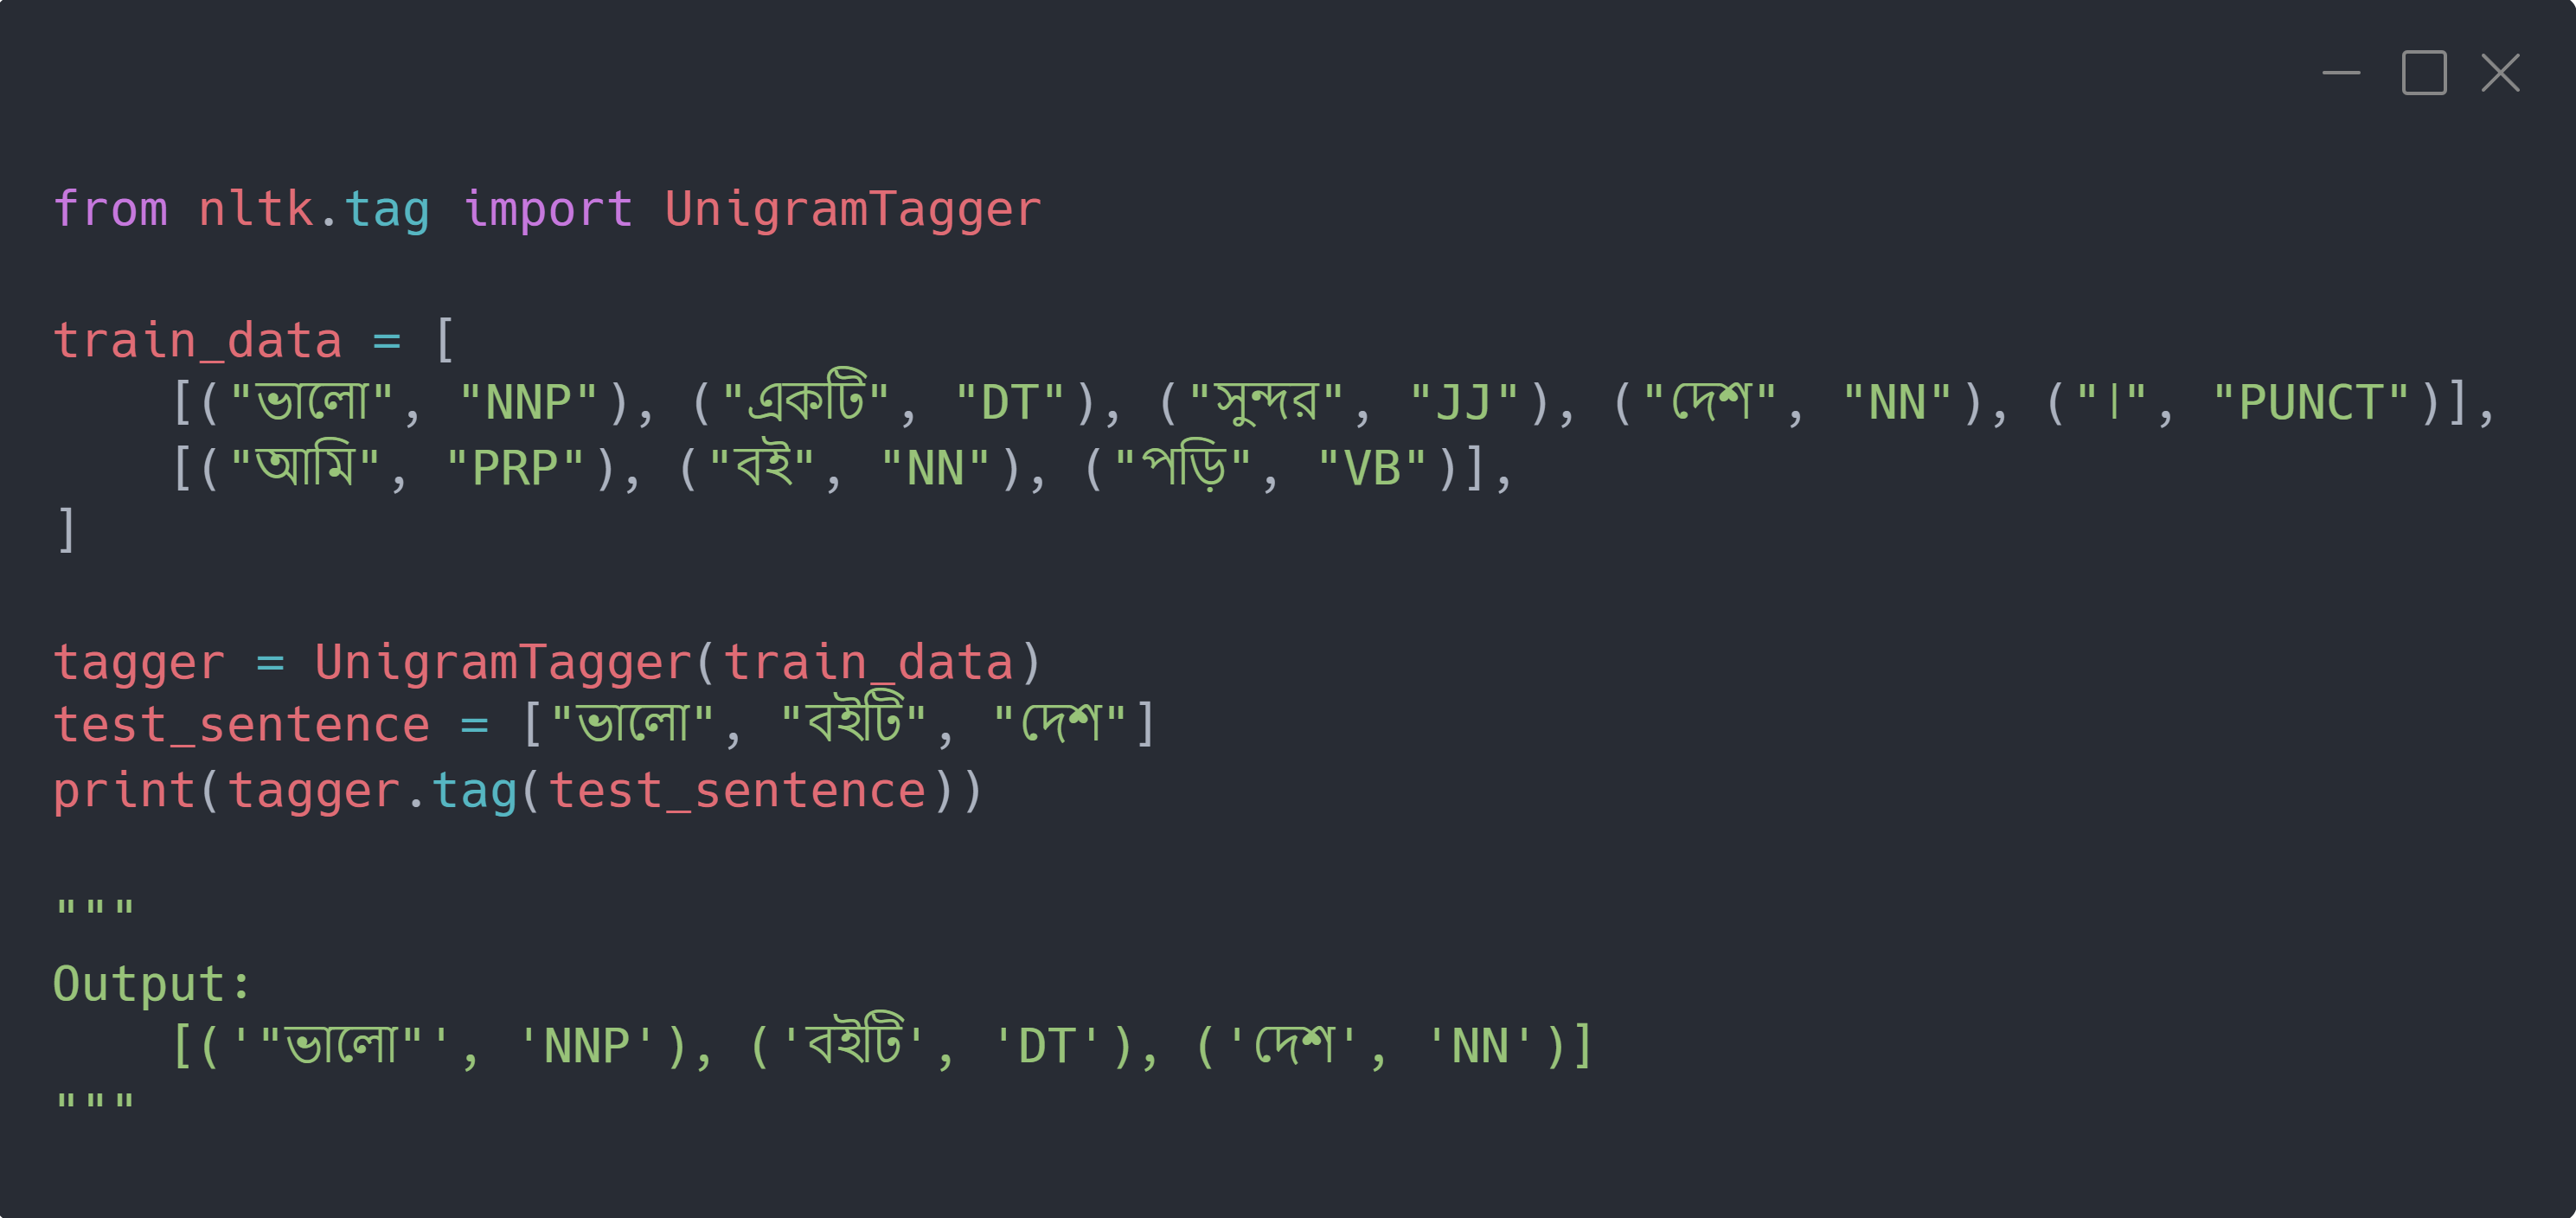
\includegraphics[width=0.8\linewidth]{Attachments/Figures/part-of-speech_figure1.png}
    \caption{Illustration of POS tagging in Bengali text.}
\end{figure}